\chapter{MPAS-Albany Land Ice Introduction}
\label{chap:landice-intro}

\section{Background}

During the past decade, numerical ice sheet models (ISMs) have undergone a renaissance relative to their predecessors. This period of intense model development was initiated following the Fourth Assessment Report of the Intergovernmental Panel on Climate Change \citep{IPCCWG1PhysicalSolomon2007}, which pointed to deficiencies in ISMs of the time as being the single largest shortcoming with respect to the scientific community's ability to project future sea-level rise stemming from ice sheets. 
Model maturation during this period, which continued through the IPCC's Fifth Assessment Report \citep{IPCCWG1PhysicalStocker2013} and to the present day, has focused on improvements to ISM ``dynamical cores'' (including the fidelity, discretization, and solution methods for the governing conservation equations \citep[e.g.,][]{Bueler2009,Schoof2010,Goldberg2011a,perego2012,Leng2012,Larour2012,Aschwanden2012,Cornford2013,gagliardini2013,brinkerhoff2013}), ISM model ``physics'' (for example, the addition of improved models of basal sliding coupled to explicit subglacial hydrology \citep[e.g.,][]{Schoof2005,Werder2013,Hewitt2013,Hoffman2014,Bueler2015}; and ice damage, fracture, and calving \citep[e.g.,][]{Astrom2014,Bassis2015,Borstad2016,Jimenez2017}) and the coupling between ISMs and Earth System Models (ESMs) \citep[e.g.,][]{Ridley2005,vizcaino2008,Vizcaino2009,Fyke2011,Lipscomb2013}. These ``next generation'' ISMs have been applied to community-wide experiments focused on assessing (i) the sensitivity of ISMs to idealized and realistic boundary conditions and environmental forcing and (ii) the potential future contributions of ice sheets to sea-level rise \citep[see e.g.,][]{pattyn2013,Nowicki2013a,Nowicki2013b,Bindschadler2013,Shannon2013,edwards2014}. 

While these efforts represent significant steps forward, next-generation ISMs continue to confront new challenges. These come about as a result of (1) applying ISMs to larger (whole-ice sheet), higher-resolution (regionally $O$(1 km) or less), and more realistic problems, (2) adding new or improved sub-models of critical physical processes to ISMs, and (3) applying ISMs as partially or fully coupled components of ESMs. The first two challenges relate to maintaining adequate performance and robustness, as increased resolution and/or complexity have the potential to increase forward model cost and/or degrade solver reliability. The latter challenge relates to the added complexity and cost associated with optimization workflows, which are necessary for obtaining model initial conditions that are realistic and compatible with forcing from ESMs. %(See related discussion in \cite{perego2014}). 
These challenges argue for ISM development that specifically targets the following model features and capabilities: 
\begin{enumerate}

\item parallel, scalable, and robust, linear and nonlinear solvers

\item variable and / or adaptive mesh resolution 

\item computational kernels based on flexible programming models, to allow for implementation on a range of High-Performance Computing (HPC) architectures\footnote{For example, traditional CPU-only architectures and MPI programming models versus CPU+GPU, hybrid architectures using MPI for nodal communication and OpenMP or CUDA for on-node parallelism.}

\item adjoint capabilities for use in high-dimensional parameter field optimization and uncertainty quantification 

\end{enumerate}

Based on these considerations, we have developed MPAS-Albany Land Ice (MALI), which is composed of three major components: 
1) model framework, 2) dynamical cores for solving equations of conservation of momentum, mass, and energy, and 3) modules for additional model physics. The model leverages existing and mature frameworks and libraries, namely the Model for Prediction Across Scales (MPAS) framework and the Albany and Trilinos solver libraries. These have allowed us to take into consideration and address, from the start, many of the challenges discussed above.
The model is described in detail in the following sections.  
MPAS-Albany Land Ice is described by a model description paper currently in review in Geoscientific Model Descriptions at:
\url{https://www.geosci-model-dev-discuss.net/gmd-2018-78/}
Much of the information in this User's Guide is derived from the text of that paper.
The User's Guide is further updated at the model evolves.


\section{MALI Meshes}

MALI typically uses centroidal Voronoi meshes on a plane.  
Spherical Voronoi meshes can also be used, but little work has been done with such meshes to date. 
Tools for creating and manipulating meshes are not yet publicly available.
MALI employs a C-grid discretization \citep{Arakawa1977} for advection, meaning state variables (ice thickness and tracer values) are located at Voronoi cell centers,
and flow variables (transport velocity, $u_n$) are located at cell edge midpoints (Figure \ref{fig:cellDiagram}).
MALI uses a sigma vertical coordinate (specified number of layers, each with a spatially uniform layer thickness fraction, see \citep{Petersen2015} for more information):
\begin{equation}
\sigma = \frac{s-z}{H}
\label{eq:sigma}
\end{equation}
where $s$ is surface elevation, $H$ is ice thickness, and $z$ is the vertical coordinate. 
Table \ref{table:meshes} describes the relationship between the MPAS Voronoi grid and the Delaunay Triangulation used by the Albany First Order velocity solver.

\begin{figure}[h]
\centering
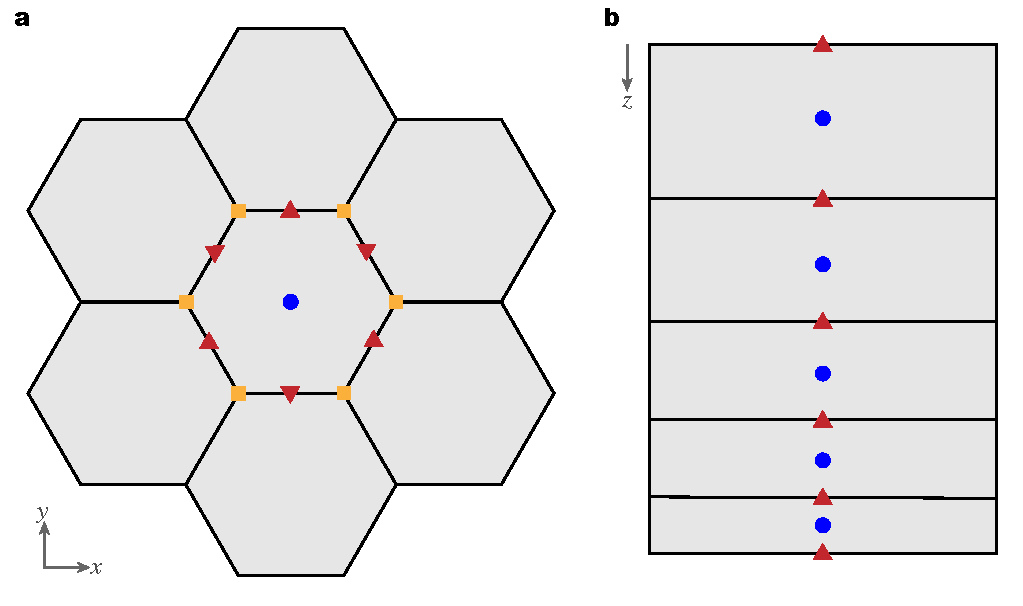
\includegraphics[width=8.3cm]{landice/figures/mpas_grids.pdf}
\caption{MALI grids.  
a) Horizontal grid with cell center (blue circles), edge midpoint (red triangles), and vertices (orange squares) identified for the center cell. Scalar fields ($H$, $T$) are located at cell centers.  Advective velocities ($u_n$) and fluxes are located at cell edges.
b) Vertical grid with layer midpoints (blue circles) and layer interfaces (red triangles) identified.  
Scalar fields ($H$, $T$) are located at layer midpoints.  Fluxes are located at layer interfaces.
}
\label{fig:cellDiagram}
\end{figure}


\begin{table*}[h]
\caption{Correspondence between the MPAS Voronoi tesselation and its dual Delaunay triangulation used by Albany.
Key MALI model variables that are natively found at each location are listed.  Note that variables are interpolated from 
one location to another as required for various calculations.
}
\begin{tabular}{lll}
\hline
Voronoi tesselation & Delaunay triangulation & Variables\\
\hline
cell center & triangle node   & $H, T, u, v$, $\Phi$ (MPAS) \\
cell edge   & triangle edge   & $u_n$ (for advection) \\
cell vertex & triangle center & $\Phi$ (Albany)\\
\hline
\end{tabular}
\label{table:meshes}
\end{table*}




\section{Albany velocity solver}
MPAS-Albany Land Ice can optionally be compiled with support for the Albany First Order velocity solver.
Albany is an open source, C++ multi-physics code base for the solution and analysis of coupled systems of partial-differential equations (PDEs) \citep{Salinger2016}. 
It is a finite element code that can (in three spatial dimensions) employ unstructured meshed comprised of hexahedral, tetrahedral, or prismatic elements. 
Albany is designed to take advantage of the computational mathematics tools available within the Trilinos suite of software libraries \citep{Trilinos} 
and it uses template-based generic programming methods to provide extensibility and flexibility \citep{Pawlowski2012}. 
Together, Albany and Trilinos provide parallel data structures and I/O, discretization and integration algorithms, 
linear solvers and preconditioners, nonlinear solvers, continuation algorithms, and tools for automatic differentiation (AD) and optimization. 
By formulating a system of equations in the residual form, Albany employs AD to automatically compute the Jacobian matrix, 
as well as forward and adjoint sensitivities. 
Albany can solve large-scale PDE-constrained optimization problems, using Trilinos optimization package ROL, 
and it provides uncertainty quantification capabilities through the Dakota framework \citep{Adams2013}. 
It is a massively parallel code by design and recently it has been adopting the Kokkos \citep{kokkos2014} programming model 
to provide manycore performance portability \citep{demeshko2018} on major HPC platforms. 
Albany provides several applications including LCM (Laboratory for Computational Mechanics) for solid mechanics problems, 
QCAD (Quantum Computer Aided Design) for quantum device modeling, and LI (Land Ice) for modeling ice sheet flow. 
We refer to the code that discretizes these ice sheet diagnostic momentum balance equations as Albany-LI.
Albany-LI was formerly known as Albany/FELIX (Finite Elements for Land Ice eXperiments), and described by 
\cite{tezaur2015a,tezaur2015b} and \cite{Tuminaro2016} under that name.

To compile MALI with support for Albany capabilities requires an installation of the Albany libraries.
Installations exist on many Department of Energy supercomputers.
To build them yourself, review the information at \url{https://github.com/gahansen/Albany/wiki}.
Compiling Albany requires a build of Trilinosi (\url{https://github.com/trilinos/Trilinos}) with specific packages and third party libraries,
and is not a trivial exercise.
Compiling Albany for usage with MPAS requires setting the Albany cmake configuration variable {\tt ENABLE\_MPAS\_INTERFACE:BOOL=ON}.
A successful Albany installation will include the file {\tt export\_albany.in}.  
Before compiling MPAS, the environment variable {\tt MPAS\_EXTERNAL\_LIBS} should be set to the list of libraries listed in this file.
Then, MALI with Albany support is enabled by compiling with {\tt ALBANY=true}, e.g.:

{\tt make gfortran CORE=landice ALBANY=true}

For MALI runs using the Albany velocity solver ({\tt config\_velocity\_solver='FO'}), an Albany .xml configuration file named {\tt albany\_input.xml}
is required in addition to the standard MPAS namelist and streams configuration files.
Examples of that file exist in the MPAS repository within subdirectories for various tests in the {\tt testing\_and\_setup/compass/landice} directory.
For further details on compiling Albany and configuring run-time options for Albany, see  \url{https://github.com/gahansen/Albany}.
